\documentclass[conference]{IEEEtran}

\usepackage{cite}
\usepackage[pdftex]{graphicx}
\graphicspath{{./figures/}}
\usepackage[cmex10]{amsmath}
\usepackage{array}
\usepackage{siunitx}
\sisetup{detect-all} % use text font instead of math font

% correct bad hyphenation here
\hyphenation{op-tical net-works semi-conduc-tor}

\begin{document}
\title{Near-Threshold Computing Revisited}

\author{\IEEEauthorblockN{Chris Gonzales\\ Mario Lok\\ Judson Porter}}
%\IEEEauthorblockA{School of Electrical and\\Computer Engineering\\
%Georgia Institute of Technology\\
%Atlanta, Georgia 30332--0250\\
%Email: http://www.michaelshell.org/contact.html}
%\and
%\IEEEauthorblockN{Homer Simpson}
%%\IEEEauthorblockA{Twentieth Century Fox\\
%%Springfield, USA\\
%%Email: homer@thesimpsons.com}
%\and
%\IEEEauthorblockN{James Kirk\\ and Montgomery Scott}
%\IEEEauthorblockA{Starfleet Academy\\
%San Francisco, California 96678-2391\\
%Telephone: (800) 555--1212\\
%Fax: (888) 555--1212}}

% make the title area
\maketitle


\begin{abstract}
%\boldmath
The abstract goes here.
\end{abstract}

\section{Introduction}
\label{sec:intro}

Power consumption and heat removal have become two of the top concerns in the datacenter space\cite{EPA_2007}. 
According to the International Technology Roadmap for Semiconductors, power consumption for each generation of chips is growing, making it one of the most significant roadblocks to future scaling \cite{Devised_2009}. 

One recently proposed  solution to this increased power is to operate the microprocessor at a significantly lowered voltage, approaching the transistor threshold voltage~\cite{Dreslinski:2010ez}. 
This near-threshold computing~(NTC) will yield approximately a 10x energy savings at the cost of 10x performance loss and a 20x total performance uncertainty. 
The NTC proposal claimed that many of these downsides can be mitigated by techniques such as device optimizations, variation tolerant circuit design, and body biasing as well as architectural changes such as increased parallelism and a move to a clustering-based architecture.

We have shown that many of the ideas presented in Dreslinski's NTC paper \cite{Dreslinski:2010ez} are ineffective at recovering the performance lost due to near-threshold computing, especially in the context of a datacenter environment. 
Although datacenters have a strong motivation to reduce their power consumption, the performance sacrifices inherent to NTC makes it an impractical choice for future servers.

In Section~\ref{sec:deltavth}, we will introduce an expression for the dependency of delay on operating voltage in near-threshold, showing that small variations in supply or threshold voltages can lead to large differences in performance.
%Section~\ref{sec:deviceoptimization} will expand upon this to show that the potential device optimizations cited by Dreslinski's NTC paper as methods to increase transistor speed will be ineffective in the near-threshold regime.
Expanding on these concerns over variability, Section~\ref{sec:criticalpaths} derives a conservative model for how the number of potential critical paths increases due to the additional delay variation inherent in near-threshold computing and Section~\ref{sec:softedge} raises concerns about the ability of soft-edge flip flops to overcome delay variations in near-threshold designs.
Section~\ref{sec:regulators} discusses power delivery concerns, both in terms of supply noise and regulator inefficiency. 
Concerns about the methodology of Dreslinski's proposed clustering architecture are addressed in Section~\ref{sec:clustering}, which is generalized in Section~\ref{sec:darksilicon} to show that any parallel architecture will have problems regaining performance lost to NTC.


\section{Near-Threshold Parallel Architectures} \label{sec:clustering}

Deslinkski et al.~\cite{dreslinski2010near} claim ``In applications where there
is an abundance of thread-level parallelism the intention is to use 10 s to 100
s of NTC processor cores that will regain 10-–50X of the performance, while
remaining energy efficient.'' In order to regain the performance lost from using
near-threshold techniques, Zhai et al.~\cite{Zhai:2007kn} and Dreslinski et
al.~\cite{Dreslinski:2007id} present a technique for leveraging parallelism in
the NTC regime. The proposed architecture groups multiple slower-cores into
clusters which share a faster L1 cache. The cache operates at $n$ times higher
frequency than the cores, where $n$ is the number of cores in a cluster. This is
motivated by the observation that SRAM has a higher energy optimal $V_{dd}$ and
$V_{th}$ than logic due to its lower activity factor and higher leakage energy
component. As a result of SRAMs higher energy optimal $V_{dd}$, the energy
optimal frequency of memory is higher than that of logic.  Based on this
observation, the proposed technique shares the first-level cache with multiple,
slower cores allowing individual tuning of $V_{dd}$ and $V_{th}$ between the
cores and memory. Using this architecture, the cores still maintain single-cycle
memory accesses while the core and memory can each operate at their energy
optimal $V_{dd}$ and $V_{th}$. Running the memory at a higher $V_{dd}$ also help
mitigate many of the reliability issues affecting SRAM in the near-threshold
regime.

Using this technique, a 71\% energy savings over a baseline single core machine
on the highly parallel SPLASH2 benchmark is demonstrated. However, in
investigating these claims, some shortcomings with this approach are revealed.
Of primary concern is the large area overhead required to achieve the same
benchmark performance. In order to achieve the same performance as a single core
baseline system, 6 cores and 3 times the baseline amount of cache were required.
It is important to remember that these results are being presented in comparison
to a single core reference on a highly parallel workload. By Amdahl's law, the
speedup from parallelism will have diminishing returns as more cores are added.
The corollary is that the biggest benefit from parallelism will be realized by
going from a single core to several cores.  It would require a larger number of
cores to achieve the same level of parallelism when comparing with a baseline
system that included more than a single core. In fact, to achieve the same
performance as the baseline, some benchmarks require as many as 16 cores and 32
times as much L1 cache (\SI{2}{\mega\byte} vs \SI{64}{\kilo\byte}). Their
results show very little energy efficiency improvement when moving from a
traditional $V_{dd}$ scaled CMP to a clustered architecture without $V_{th}$
tuning.

The clustering technique also uses separate $V_{th}$ tuning for the core and
cache to find the energy optimal voltage for the same performance. However, in
examining what these voltages actually are, it is revealed that neither $V_{dd}$
of the cache nor the logic is actually in the near-threshold regime as defined
by the paper, and both are in fact operating at a $V_{dd}$ 2x--3x higher than
the selected $V_{th}$. In modern process technologies, the standard is $V_{dd}$
already approaching 2x $V_{th}$. As described in Section~\ref{sec:bodybiasing},
the techniques for tuning $V_{th}$ are also becoming less effective.

One final concern is that while energy optimal cluster configurations are
presented for each SPLASH2 benchmark, no co-optimized configuration is given.
This could potentially be an issue as the energy optimal range of cores,
clusters, cache sizes, $V_{dd}$ and $V_{th}$ is large. It is unclear what the
energy savings across benchmarks for different configurations will be.

\section{Shortcomings of Application Parallelism} \label{sec:darksilicon}

Dreslinski et al.~\cite{Dreslinski:2010ez} state ``More gates can now fit on a die, but a growing fraction cannot actually be used due to strict power limits.''
This issue is commonly referred to as dark silicon.
While the number of transistors on a given die has been doubling every generation, the number of transistors that can be powered for a fixed power budget has not been increasing due to the slowing of transistor energy scaling.
Since power budgets have not been increasing, a situation has arisen where future generations of chips will potentially have more transistors than can be powered at any given time.

Dark silicon seemingly presents an opportunity for near-threshold computing, and as a way of addressing the large area overheads of the clustering architectures discussed in Section~\ref{sec:clustering}.
By reducing the power consumed per-core, more cores can be simultaneously powered.
Since these cores could not be powered in a super-threshold chip, this represents an opportunity for near-threshold chips to regain performance compared to super-threshold operation.

\begin{figure}[thpb] \centering
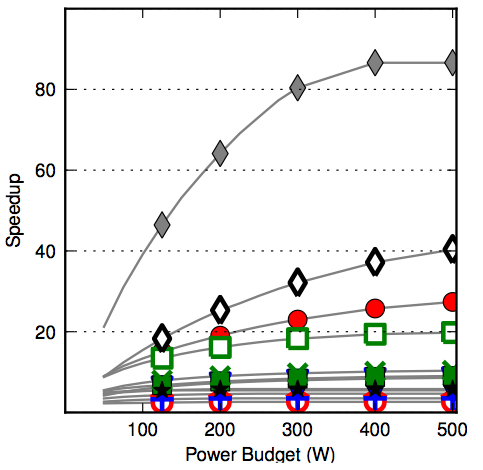
\includegraphics[width=0.3\textwidth]{esmaeilzadeh_power_speedups.png}
\caption{Projected speedups on PARSEC benchmarks while the chip power limit (and therefore the number of cores) is increased.~\cite{Esmaeilzadeh2011Dark-silicon-an}}
\label{fig:power_speedups}
\end{figure}

While dark silicon is an opportunity for devices to reach higher levels of integration, recent studies analyzing dark silicon have not borne out the promise of higher levels of performance with increasing core counts.
Esmaeilzadeh et. al~\cite{Esmaeilzadeh2011Dark-silicon-an} developed an analytical model analyzing the impact of dark silicon for a range of CMP configurations in future process technologies.
They show projected speedups for these configurations using the PARSEC benchmark suite, which represents workloads similar to the SPLASH2 benchmark suite used in clustering architecture discussed in Section~\ref{sec:clustering}, indicating that both works are targeting similar application spaces.
This analytical model does project that dark silicon will become a significant portion of CPU area in the near future, dominating as soon as 2016 with a conservative scaling model.
The authors also analyze the case where the power constraint is lifted, which allows more cores to be powered and reduces the amount of dark silicon.
Figure~\ref{fig:power_speedups} shows the projected speedups on different PARSEC benchmarks as the chip power is increased.
The paper projects that if the amount of parallelism in applications were increased to 99\%, then the best case speedup for power limited cores in \SI{8}{\nano\meter} is 15x relative to a quad-core Nehalem processor at \SI{45}{\nano\meter}.
However, 8 out of 12 PARSEC benchmarks achieve no more than 10x speedup with an unconstrained power budget, as shown in Figure~\ref{fig:power_speedups}. 
This indicates that the amount of parallelism in general-purpose parallel workloads will be exploitable even by future power constrained multi-core chips.
While near-threshold computing would allow more chips to be powered, it would not realize a significant speedup on most general-purpose parallel workloads due to the lack of exploitable parallelism.

\begin{figure}[thpb]
\centering
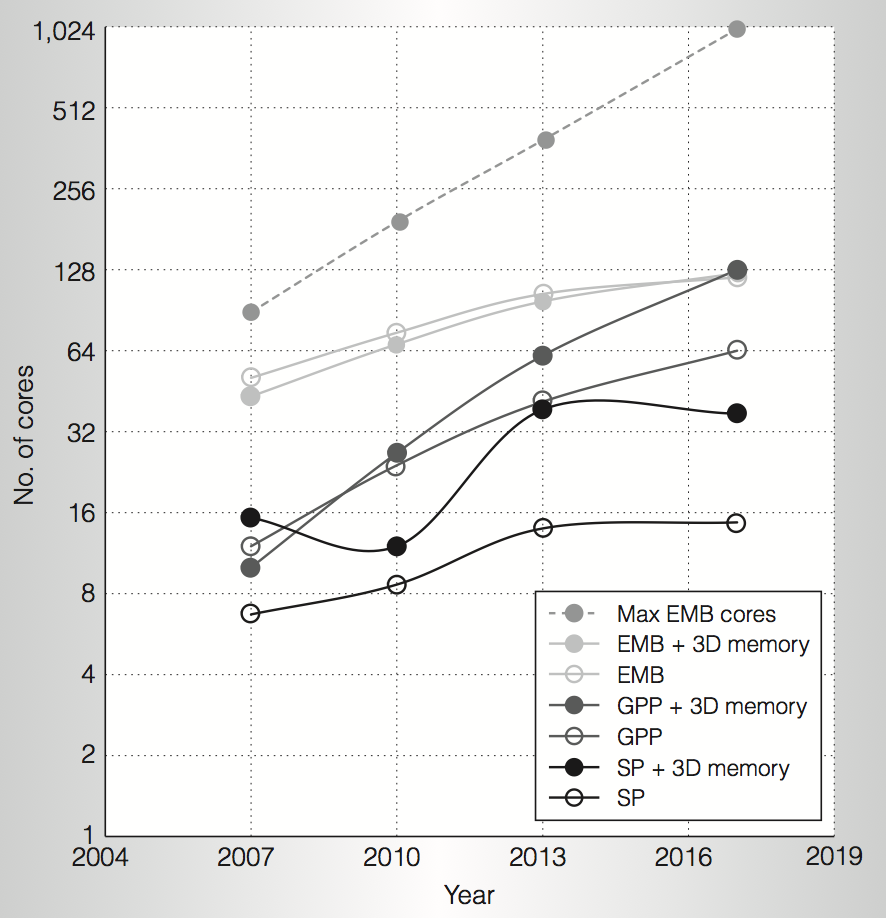
\includegraphics[width=0.4\textwidth]{hardavellas_core_counts.png}
\caption{Projections for core count scaling.~\cite{Hardavellas:2011de}}
\label{fig:core_counts}
\end{figure}

\begin{figure}[thpb]
\centering
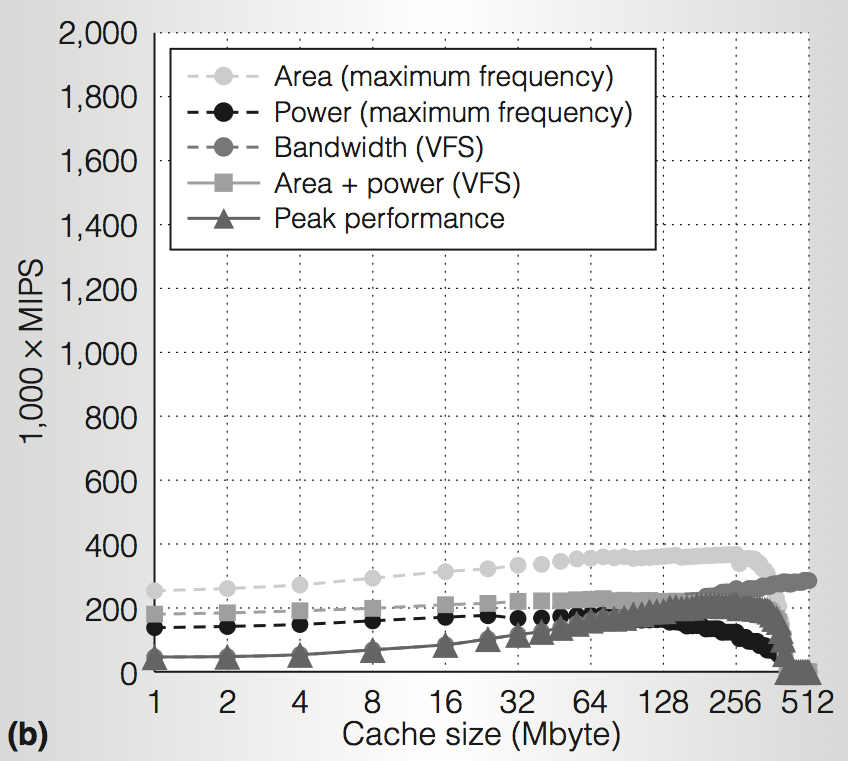
\includegraphics[width=0.4\textwidth]{hardavellas_emb_performance.png}
\caption{Embedded core scaling.~\cite{Hardavellas:2011de}}
\label{fig:emb_performance}
\end{figure}

Further work by Hardavellas et al.~\cite{Hardavellas:2011de} confirms the observation that future speedups are limited by application level parallelism, not power constraints.
In this study the authors built an analytical chip performance model for different types of cores, including low-power embedded cores (EMBs) similar to an ARM11 MPCore, and modeled how the performance of these chips scale in future process technologies given area, power, and memory bandwidth constraints.
Figure~\ref{fig:core_counts} shows projected core count scaling trends in future process technologies.
The difference between the ``Max EMB cores'' line and the ``EMB'' line represents the difference in how many cores can fit on a die versus how many can be powered given current chip power constraints.
Their model projects that in 2017 over 1024 cores will be able to fit on a die, but only 12\% of them will be able to be powered at any given time.
Again, this looks like an opportunity for near-threshold computing to increase core counts over traditional super-threshold CMPs.

Figure~\ref{fig:emb_performance} shows the maximum performance of an EMB-based CMP given different constraints for a 99\% parallel workload.
The ``Area (maximum frequency)'' line represents the best performance with only a die area constraint, while the ``Peak Performance'' line represents the best performance factoring in area, power, and memory bandwidth constraints.
While the constrained case only has 12\% of the cores of the area constrained case, it only has approximately half the performance of the unconstrained case.
Again, the performance is limited by the application parallelism, not the number of cores integrated onto the chip.

While NTC processors could support increased core counts over super-threshold chips, they would not be able to gain back a significant amount of the performance loss as super-threshold core counts are already approaching the limits of exploitable parallelism in general-purpose workloads.
Without a focus on increasing the amount of parallelism in these applications, opportunities for NTC processors to regain performance loss through parallelism will be limited.

\section{Conclusion}
\label{sec:conclusion}

In the general-purpose server computing space, near-threshold computing is not a viable solution to achieving more energy efficiency computing while maintaining system throughput.
The inherent problems of slower devices and increased variability in near-threshold computing are still major barriers for a near-threshold server processor to achieve the same throughput level as a super-threshold server processor.
The state-of-the-art device optimization for low voltage operation provides little performance boost to transistors operating in the near-threshold region.
Soft-edge clocking becomes less effective in combating variation in near-threshold.Adding to the difficulties of applying near-threshold computing, the inefficiency of delivering power to a low voltage chip and the stricter requirement on the power supply diminishes the power reduction benefits from operating the server processor at low voltage.
Worst of all, the marginal parallelism that can be extracted from the already highly parallel server workload is far from enough to bridge the 10X performance gap between near-threshold computing and traditional above threshold computing.


\bibliographystyle{IEEEtran}
\bibliography{IEEEabrv,bibtex}

\end{document}


